%\pagestyle{fancy}
%\thispagestyle{plain}
%\pagestyle{fancyplain}
%\lhead[\fancyplain{}{\slshape %\rightmark}]
%\chead{}
%\rhead[\fancyplain{}{\slshape %\leftmark}]
%\lfoot[]{\thepage}
%\cfoot[]{Estadistica I}
%\rfoot{\thepage}
%\setlength{\headrulewidth}{0.4pt}
%\setlength{\footrulewidth}{0.4pt}
%TCIDATA{OutputFilter=latex2.dll}
%TCIDATA{Version=4.00.0.2312}
%TCIDATA{LaTeXparent=0,0,Est12.tex}
%TCIDATA{ChildDefaults=%
%chapter:4,page:103
%}


\section{Variables aleatorias}

\section{}

\begin{itemize}
\item Variable aleatoria discreta. Si toma un n\'{u}mero finito o numerable de
valores, por ejemplo
\[
X:\longrightarrow\nz
\]


\item Variable aleatoria continua. Si toma un n\'{u}mero de valores no
numerables, por ejemplo
\[
X:\longrightarrow\rz
\]

\end{itemize}

\section{Variables aleatorias discretas}



\begin{definition}
Si $X$ es una variable aleatoria discreta, asociamos un n\'{u}mero
\[
f\left(  x_{i}\right)  =P\left(  X=x_{i}\right)
\]
como cada resultado $x_{i}$ en $R_{X}$ para $i=1,2,3\cdots,n,\cdots,$ donde
los n\'{u}meros $f\left(  x_{i}\right)  $ satisfacen

\begin{enumerate}
\item $f\left(  x_{i}\right)  \geq0\quad$para toda $i$

\item $\sum_{i=1}^{x}f\left(  x_{i}\right)  =1$

La funci\'{o}n $f\left(  x_{i}\right)  $ se llama funci\'{o}n de probabilidad
o ley de probabilidad de la variable aleatoria, y la colecci\'{o}n de pares
$\left(  x_{i},f\left(  x_{i}\right)  \right)  $ se llama distribuci\'{o}n de
probabilidad de $X$

\item Dada una variable aleatoria discreta $X:S\longrightarrow\nz $, su
funci\'{o}n de probabilidad $f$ se define de modo que $f\left(  x_{i}\right)
$ es la proba\-bilidad de que $X$ tome ese valor
\[
\begin{array}
[c]{ccc}%
f:\nz & \longrightarrow & [0,1]\\
x_{i} & \longmapsto & f\left(  x_{i}\right)  =P\left(  X=x_{i}\right)
\end{array}
\]
si $x_{i}$ no es uno de los valores que puede tomar $X$, entonces $f\left(
x_{i}\right)  =0$
\end{enumerate}
\end{definition}

\begin{definition}
[Funci\'{o}n de distribuci\'{o}n]De una variable alea\-toria discreta, $F$ que
se define de modo que si $x_{i}\in\rz ,F\left(  x_{i}\right)  $ es igual a la
probabilidad de que $X$ tome un valor inferior o igual a $x_{i}$, es decir,
\[
\begin{array}
[c]{ccc}%
F:\nz & \longrightarrow & [0,1]\\
x_{i} & \longmapsto & F\left(  x_{i}\right)  =P\left(  x_{i}\geq X\right)
\end{array}
\]

\end{definition}

\begin{remark}
La funci\'{o}n de distribuci\'{o}n $F$, es una funci\'{o}n no decreciente, es
decir. Si
\[
x_{1<}x_{2}\Longrightarrow F\left(  x_{2}\right)  \geq F\left(  x_{1}\right)
\]
Adem\'{a}s, es continua a la derecha
\[
\lim_{x\longrightarrow a^{+}}F\left(  x\right)  =F\left(  a\right)
\]
y
\begin{align*}
F\left(  -\infty\right)   &  =\lim_{x\longrightarrow-\infty}F\left(
x_{i}\right)  =0\\
F\left(  +\infty\right)   &  =\lim_{x\longrightarrow+\infty}F\left(
x_{i}\right)  =1
\end{align*}

\end{remark}

\begin{example}
Sup\'{o}ngase que tenemos una variable aleatoria $X$ con una distribuci\'{o}n
de probabiliadad dada por la relaci\'{o}n
\[
f\left(  x\right)  =\left\{
\begin{array}
[c]{cc}%
\binom{n}{x}p^{x}\left(  1-p\right)  ^{n-x} & x=0,1,2,...,n\\
0 & \text{de otro modo}%
\end{array}
\right.
\]
donde n es un entero positivo y $0\leq p\leq1.$ El ejemplo anterior es un caso
pareticular de \'{e}sta distribuci\'{o}n de probabilidad llamada Binomial
\end{example}

\section{Variables aleatorias continuas}



Cuando tenemos una variable\ aleatoria continua no tiene sentido realizar una
suma de las probabilidades de cada uno de los valores que toma, ya que el
conjunto es no enumerable por lo que hay que introducir otro concepto.

Sea $f:\rz\longrightarrow\rz$ una funci\'{o}n llamada funci\'{o}n de densidad
de una variable aleatoria continua, integrable que cumple las propieda\-des
\begin{align*}
f\left(  x\right)   &  \geq0\\
\int_{-\infty}^{+\infty}f\left(  x\right)  dx &  =1
\end{align*}
adem\'{a}s para todo $[a,b]$ se tiene
\[
P\left(  a\leq x\leq b\right)  =\int_{a}^{b}f\left(  x\right)  dx
\]
%

%TCIMACRO{\FRAME{dtbpFU}{3.6097in}{1.9104in}{0pt}{\Qcb{Funci\'{o}n de densidad
%de $f\left(  x\right)  $}}{\Qlb{fig 4.5}}{img813.wmf}%
%{\special{ language "Scientific Word";  type "GRAPHIC";
%maintain-aspect-ratio TRUE;  display "USEDEF";  valid_file "F";
%width 3.6097in;  height 1.9104in;  depth 0pt;  original-width 7.7038in;
%original-height 4.0517in;  cropleft "0";  croptop "1";  cropright "1";
%cropbottom "0";  filename '../Tacho/img813.wmf';file-properties "XNPEU";}}}%
%BeginExpansion
\begin{center}
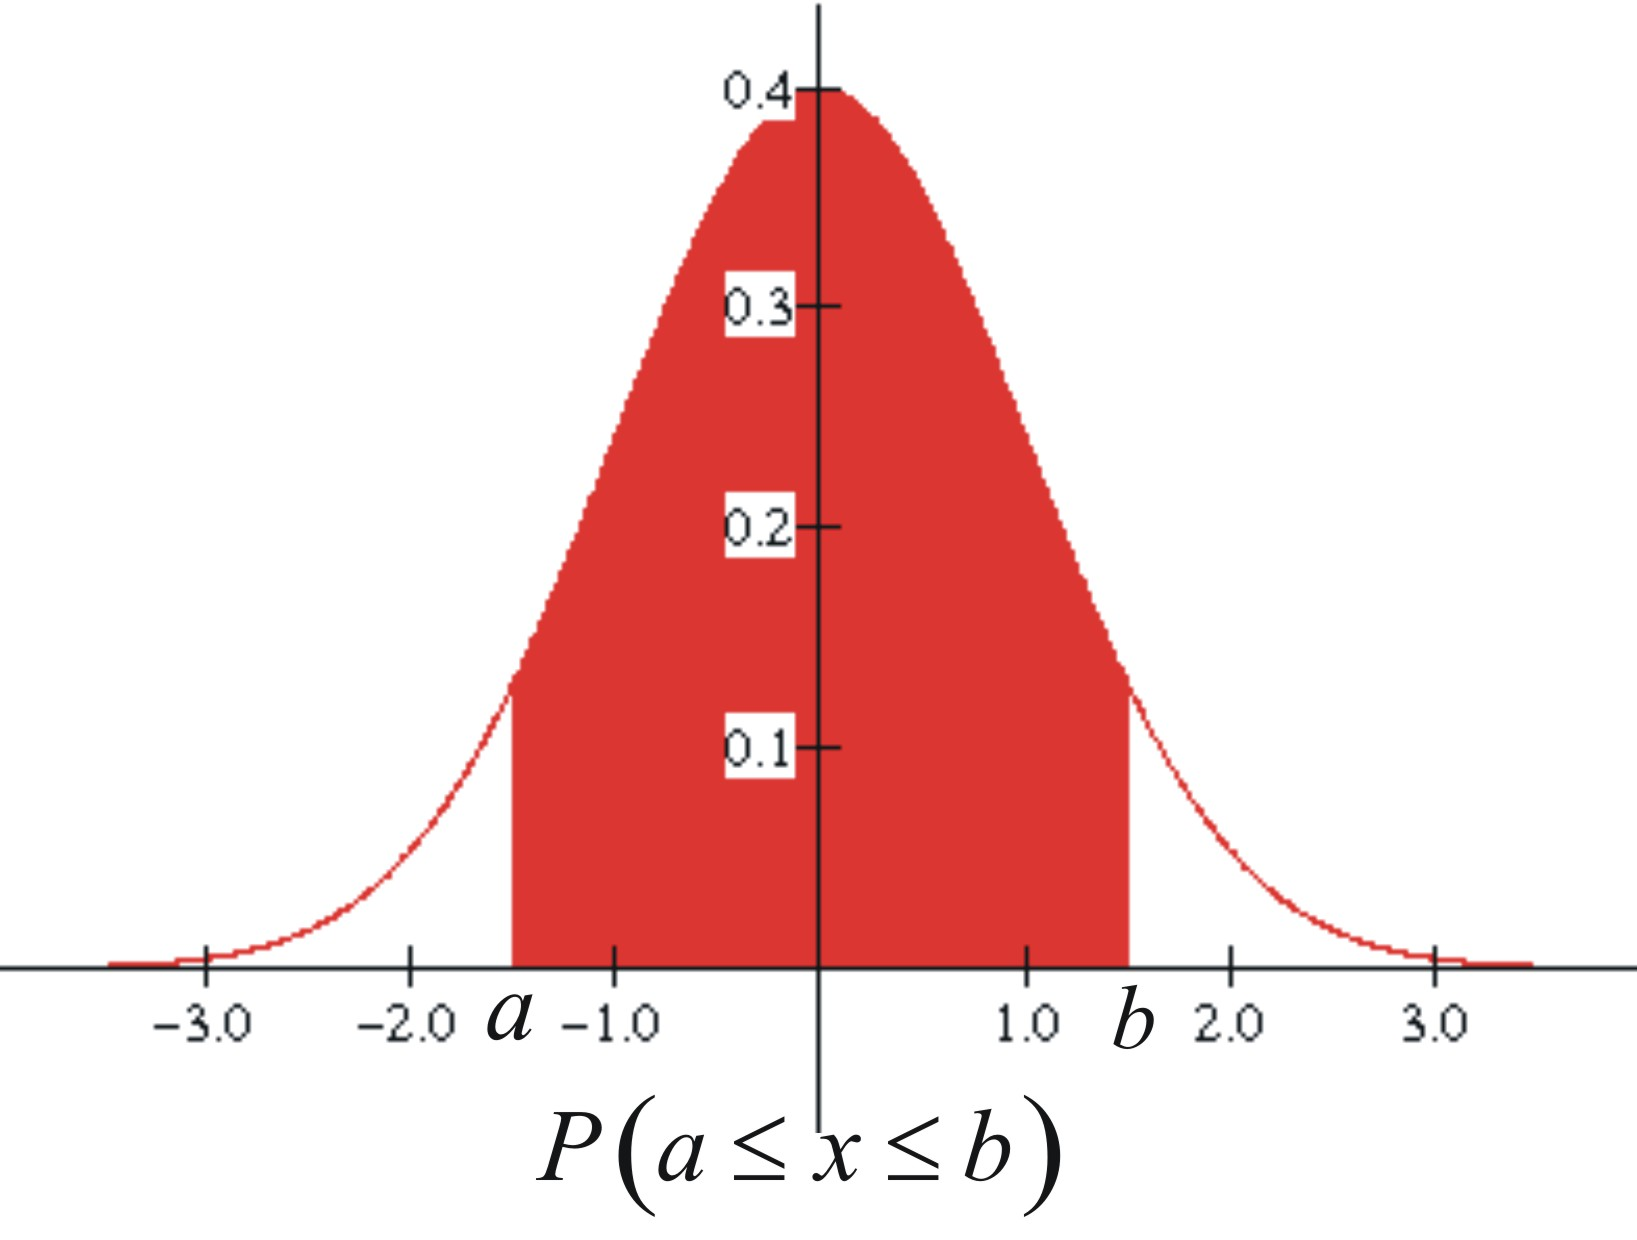
\includegraphics[width=7cm]{img813.jpg}
\label{fig4.5}
\end{center}

%EndExpansion


\begin{remark}
Al observar la gr�fica vemos que $P\left(  a\leq x\leq b\right) $
es el \'{a}rea bajo la curva de $f$
\end{remark}

\begin{remark}
Por ser $f$ integrable entonces la la probabilidad en un punto es nula, es
decir
\[
P\left(  X=a\right)  =P\left(  a\leq x\leq a\right)  =\int_{a}^{a}f\left(
x\right)  dx=0
\]

\end{remark}

\begin{remark}
Debido a lo anterior se tiene que

\begin{itemize}
\item La funci\'{o}n de densidad no es \'{u}nica

\item $P\left(  a\leq x\leq b\right)  =P\left(  a<x<b\right)  $

\item $P\left(  a\leq x\leq b\right)  =P\left(  a\leq x<b\right)  =P\left(
a<x\leq b\right)  $
\end{itemize}
\end{remark}

La funci\'{o}n de distribuci\'{o}n de una variable aleatoria, $F,$ continua se
define de modo que dado $x\epsilon$ $\rz$, $F\left(  x\right)  $ es la
probabilidad de que $X$ sea mayor o igual que $x,$ es decir
\[
\begin{array}
[c]{ccc}%
F:\rz & \longrightarrow & [0,1]\\
x & \longmapsto & F\left(  x\right)  =P\left(  x\geq X\right)  =\int_{-\infty
}^{x}f\left(  t\right)  dt
\end{array}
\]




\begin{proposition}
Dado un intervalo de la forma $(a,b]$, tenemos
\begin{align*}
P\left(  X\in(a,b]\right)   &  =\int_{a}^{b}f\left(  x\right)  dx\\
&  =\int_{-\infty}^{b}f\left(  x\right)  dx-\int_{-\infty}^{a}f\left(
x\right)  dx\\
&  =F\left(  b\right)  -F\left(  a\right)
\end{align*}
Se puede observar que la cantidad $F\left(  b\right)  -F\left(  a\right)  $
representa la masa de probabilidad extendida alo largo del intervalo $(a,b]$ .
Si dividimos esta cantidad por la longitud del intervalo,
\[
\frac{F\left(  b\right)  -F\left(  a\right)  }{b-a}
\]
tenemos la masa media de probabilidad por unidad de longitud en $(a,b]$, es
decir, su densidad media de probabilidad, ahora si
\[
\lim_{a\longrightarrow b}\frac{F\left(  b\right)  -F\left(  a\right)  }%
{b-a}=F^{\prime}\left(  b\right)  =f\left(  b\right)
\]
que es la densidad de probabilidad en el punto $b$
\end{proposition}

\begin{remark}
\begin{itemize}
\item Si $X$ es una variable continua la funci\'{o}n de distribuci\'{o}n $F$
es no decreciente, es decir si
\[
x_{1}<x_{2}\Longrightarrow F\left(  x_{2}\right)  \geq F\left(  x_{1}\right)
\]


\item esta funci\'{o}n es absolutamente convergente y se verifica
\begin{align*}
F\left(  -\infty\right)   &  =\lim_{x\longrightarrow-\infty}F\left(  x\right)
=0\\
F\left(  +\infty\right)   &  =\lim_{x\longrightarrow+\infty}F\left(  x\right)
\left(  1\right)
\end{align*}

\end{itemize}
\end{remark}

\begin{definition}
Funciones de probabilidad bivariada

\begin{enumerate}
\item Caso discreto: para cada resultado $\left(  x_{1i},x_{2j}\right)  $ de
$\left(  X_{1},X_{2}\right)  ,$ asociamos un n\'{u}mero
\[
f\left(  x_{1i},x_{2j}\right)  =P\left(  X_{1}=x_{1i},X_{2}=x_{2j}\right)
\]
donde
\begin{align*}
f\left(  x_{1i},x_{2j}\right)   &  \geq0\text{ }\\
\text{para todo }i  &  \in I,j\in J\text{ siendo }I,J\text{ conjuntos de
sub\'{\i}ndices}%
\end{align*}
y
\[
\sum_{i\in I}\sum_{j\in J}f\left(  x_{1i},x_{2j}\right)  =1
\]
Los valores $\left(  \left(  x_{1i},x_{2j}\right)  ,f\left(  x_{1i}%
,x_{2j}\right)  \right)  $ para todo $i\in I$ y $j\in J$ forman la
distribuci\'{o}n de probabilidad de $\left(  X_{1},X_{2}\right)  $

\item Caso continuo . Si $\left(  X_{1},X_{2}\right)  $ es un vector aleatorio
continuo con espacio del rango, $R,$ en $\rz^{2}$, entonces $f$, la
funci\'{o}n de densidad conjunta, tiene las siguientes propiedades
\[
f\left(  x_{1},x_{2}\right)  \geq0\text{ }\forall\left(  x_{1},x_{2}\right)
\in R
\]
y
\[
\int\int_{R}f\left(  x_{1},x_{2}\right)  dx_{1}dx_{2}=1
\]

\end{enumerate}
\end{definition}

\begin{definition}
Se dice que $\ n$ variables aleatorias \newline$X_{1},X_{2},X_{3},\cdots
,X_{k},$tiene una distribuci\'{o}n discreta conjunta si el vector
aleatorio\newline$X=\left(  X_{1},X_{2},X_{3},\cdots,X_{k}\right)  $ puede
tomar solamente un n\'{u}mero finito o una sucesi\'{o}n finita de valores
distintos posibles$\left(  x_{1},x_{2},x_{3},\cdots,x_{k}\right)  $ en
$\rz^{k}$. La funci\'{o}n de probabilidad cunjunta \ de $X_{1},X_{2}%
,X_{3},\cdots,X_{k}$ se define entonces como la funci\'{o}n $f$ tal que para
cualquier punto $x=\left(  x_{1},x_{2},x_{3},\cdots,x_{k}\right)  \in
A\subset$\rz$^{k},$%
\[
f\left(  x\right)  =P\left(  X=x\right)  \quad\forall x\in A
\]
donde $A$ es cualquier subconjunto de $\rz^{k}$
\[
P\left(  x\in A\right)  =\sum_{x\in A}f\left(  x\right)
\]

\end{definition}

\begin{definition}
Distribuciones continuas. se dice que n varibles aleatorias $X_{1},X_{2}%
,X_{3},\cdots,X_{k}$ tienen una distribuci\'{o}n conjunta continua si existe
una funci\'{o}n no negativa f definida sobre $\rz^{k}$ tal que para cualquier
subconjunto $A\subset\rz^{k}$
\begin{align*}
&  P\left(  \left(  X_{1},X_{2},X_{3},\cdots,X_{k}\right)  \in A\right) \\
&  =\int\cdots\int_{A}f\left(  x_{1},x_{2},x_{3},\cdots,x_{k}\right)
dx_{1}dx_{2}\cdots dx_{k}%
\end{align*}

\end{definition}

\begin{definition}
La f.d conjunta de k variables aleatorias\newline$X_{1},X_{2},X_{3}%
,\cdots,X_{k},$ se define como la funci\'{o}n $F$ cuyo valor en cualquier
punto $\left(  x_{1},x_{2},x_{3},\cdots,x_{k}\right)  $ de un espacio
k-dimensional
%TCIMACRO{\TeXButton{rz}{\rz}}%
%BeginExpansion
\rz
%EndExpansion
$^{k}$ est\'{a} dado por la relaci\'{o}n
\[
F\left(  x_{1},x_{2},x_{3},\cdots,x_{k}\right)  =P\left(  X_{1}\leq
x_{1},\cdots X_{k}\leq x_{k}\right)
\]

\end{definition}

\begin{remark}
\'{E}sta f.d satisface todas las propiedades de la f.d univariada.
\end{remark}

En el caso bivariado. Si $X$ y $Y$ son variables aleatorias con f.d.p conjunta
$f$ se tiene que
\[
F\left(  x,y\right)  =\int_{-\infty}^{x}\int_{-\infty}^{y}f\left(  u,v\right)
dudv
\]


Si la disribuci\'{o}n conjunta de $X_{1},X_{2},X_{3},\cdots,X_{k}$ es
continua, entonces la f.d.p conjunta f se puede obtener a partir de la f.d
conjunta F utilizando la relaci\'{o}n
\[
f\left(  x_{1},x_{2},x_{3},\cdots,x_{k}\right)  =\frac{\partial^{k}F\left(
x_{1},x_{2},x_{3},\cdots,x_{k}\right)  }{\partial x_{1}\partial x_{2}%
\cdots\partial x_{k}}
\]
para todos los puntos $\left(  x_{1},x_{2},x_{3},\cdots,x_{k}\right)  $ donde
exista la derivada.

En el caso bivariado
\[
f\left(  x,y\right)  =\frac{\partial^{2}F\left(  x,y\right)  }{\partial
x\partial y}
\]
$\forall\left(  x,y\right)  $ donde exista la derivada parcial de 2%
%TCIMACRO{\U{ba} }%
%BeginExpansion
${{}^o}$
%EndExpansion
orden

\begin{example}
Sup\'{o}ngase que la variable aleatoria X puede tomar solamente los valores
1,2,3, y que la variable Y puede tomar solamente los valores 1,2,3,4, donde la
f.p conjunta de X e Y es como indica la tabla\newline%
\begin{tabular}
[c]{|c|c|c|c|c|}\hline
$X|Y$ & 1 & 2 & 3 & 4\\\hline
1 & 0.1 & 0 & 0.1 & 0\\\hline
2 & 0.3 & 0 & 0.1 & 0.2\\\hline
3 & 0 & 0.2 & 0 & 0\\\hline
\end{tabular}
\newline determine los valores de $P\left(  X\geq2,Y\geq2\right)  $ y
$P\left(  X=1\right)  $

\begin{solution}
Sumando$f\left(  x.y\right)  $ sobre todos los valores de $x\geq2$ y de
$y\geq2,$ se obtiene
\begin{align*}
p\left(  X\geq2,Y\geq2\right)   &  =f\left(  2,2\right)  +f\left(  2,3\right)
+f\left(  2,4\right)  +\\
&  +f\left(  3,2\right)  +f\left(  3,3\right)  +f\left(  3,4\right) \\
&  =0.5\\
P\left(  X=1\right)   &  =\sum_{y=1}^{4}f\left(  1,y\right)  =0.2
\end{align*}

\end{solution}
\end{example}

\begin{center}

\end{center}

\begin{example}
Sup\'{o}ngase que la f.d.p conjunta de x e Y es la sigui\-ente
\[
f\left(  x,y\right)  =\left\{
\begin{array}
[c]{ccc}%
cx^{2}y & para & x^{2}\leq y\leq1\\
0 &  & \text{en otro caso}%
\end{array}
\right.
\]


\begin{itemize}
\item Determine el valor de la constante c

\item $P\left(  X\geq Y\right)  $
\end{itemize}

\begin{solution}
Sea el conjunto S de puntos $\left(  x,y\right)  $ para los que f$\left(
x,y\right)  >0$ est\'{a} representado en la figura 4.8 . puesto que $f\left(
x,y\right)  =0$ fuera de S, resulta que
\[
\int\int_{s}f\left(  x,y\right)  dxdy=\int_{-1}^{1}\int_{x^{2}}^{1}%
cx^{2}ydydx=\frac{4}{21}c
\]
y como esta integral debe ser 1, entonces c=$\frac{21}{4}$\newline$%
%TCIMACRO{\FRAME{itbpFU}{2.9706in}{1.9969in}{0in}{\Qcb{fig(a) Ejemplo 4.8}%
%}{\Qlb{fig 4.8a}}{imagen4.wmf}{\special{ language "Scientific Word";
%type "GRAPHIC";  maintain-aspect-ratio TRUE;  display "USEDEF";
%valid_file "F";  width 2.9706in;  height 1.9969in;  depth 0in;
%original-width 2.9274in;  original-height 1.9579in;  cropleft "0";
%croptop "1";  cropright "1";  cropbottom "0";
%filename '../Tacho/imagen4.wmf';file-properties "XNPEU";}}}%
%BeginExpansion
{\parbox[b]{2.9706in}{\begin{center}
\includegraphics[
natheight=1.957900in,
natwidth=2.927400in,
height=1.9969in,
width=2.9706in
]%
{imagen4.png}%
\\
fig(a) Ejemplo 4.8
\end{center}}}%
%EndExpansion
$

\begin{itemize}
\item Sea S$_{0}$ el conjunto donde x$\geq y$, entonces
\begin{align*}
\int\int_{S_{0}}f\left(  x,y\right)  dxdy &  =\\
\int_{0}^{1}\int_{x^{2}}^{x}\frac{21}{4}x^{2}ydydx &  =\frac{3}{20}%
\end{align*}%
%TCIMACRO{\FRAME{dhFU}{2.9706in}{1.9969in}{0pt}{\Qcb{Fig(b) Ejemplo 4.8}%
%}{\Qlb{fig 4.8b}}{imagen47.wmf}{\special{ language "Scientific Word";
%type "GRAPHIC";  maintain-aspect-ratio TRUE;  display "USEDEF";
%valid_file "F";  width 2.9706in;  height 1.9969in;  depth 0pt;
%original-width 2.9274in;  original-height 1.9579in;  cropleft "0";
%croptop "1";  cropright "1";  cropbottom "0";
%filename '../Tacho/Imagen47.wmf';file-properties "XNPEU";}}}%
%BeginExpansion
\begin{center}
\includegraphics[width=7cm]{imagen47.jpg}
\end{center}

%EndExpansion

\end{itemize}
\end{solution}
\end{example}

\begin{itemize}
\item En el caso discreto\ la distribuci\'{o}n marginal para $X_{1}$ y $X_{2}$
es
\begin{align*}
f\left(  x_{1}\right)   &  =\sum_{todo\,j}f\left(  x_{1i},x_{2j}\right)
\,\forall i=1,2,\cdots\\
f\left(  x_{2}\right)   &  =\sum_{todo\,i}f\left(  x_{1i},x_{2j}\right)
\,\forall j=1,2,\cdots
\end{align*}


\item En el caso continuo la distribuci\'{o}n marginal para $X_{1}$ y $X_{2}$
es
\begin{align*}
f\left(  x_{1}\right)   &  =\int_{-\infty}^{\infty}f\left(  x_{1}%
,x_{2}\right)  dx_{2}\\
f\left(  x_{2}\right)   &  =\int_{-\infty}^{\infty}f\left(  x_{1}%
,x_{2}\right)  dx_{1}%
\end{align*}

\end{itemize}
